%%Standarddokument, v1.88 %%

\documentclass[a4paper,DIV=calc,11pt]{scrartcl}
\usepackage[T1]{fontenc}
\usepackage[utf8]{inputenc} %Zeichencodierung
\usepackage[ngerman]{babel} %Sprachpaket
\usepackage{setspace} % Einstellungen für den Zeilenabstand
\usepackage{libertine} % Schriftart
\usepackage[scaled=.7]{beramono}
\usepackage{microtype} %typografische Verbesserungen
\usepackage[colorlinks=false,pdfborder={0 0 0},bookmarksnumbered]{hyperref}
\usepackage{pdfpages}

\begin{document}

\hypersetup{
	pdftitle={Titel des Dokuments},
	pdfauthor={Mein Name},
	pdfsubject={Thema der Arbeit}
	}
	
%\onehalfspace % 1,5-facher Zeilenabstand
	
\title{Book Proposal}
%\subtitle{Noch ein Untertitel}
\author{Fabian Bross \\ University of Stuttgart \\ Linguistics Department \\ Keplerstraße 17 \\ 70174 Stuttgart \\ Germany}
\date{\small February 2019}
\maketitle %gibt die Titelangaben aus

\noindent Dear editors, I would like to submit the following book proposal for the series ``Open Generative Syntax''. The title of the proposed book (a revised version of my dissertation) is ``The Clausal Syntax of German Sign Language: A Cartographic Approach''. In the following you find a table of contents, a text description of the content, and abstracts of the chapters. I left out the comparison with books that are already available as I think that there are no comparable works on the Cartography of sign languages.

Note that you can take a look at the manusscript here: http://fabianbross.de/book.zip (the password is ``dgs'' without quotation marks). 



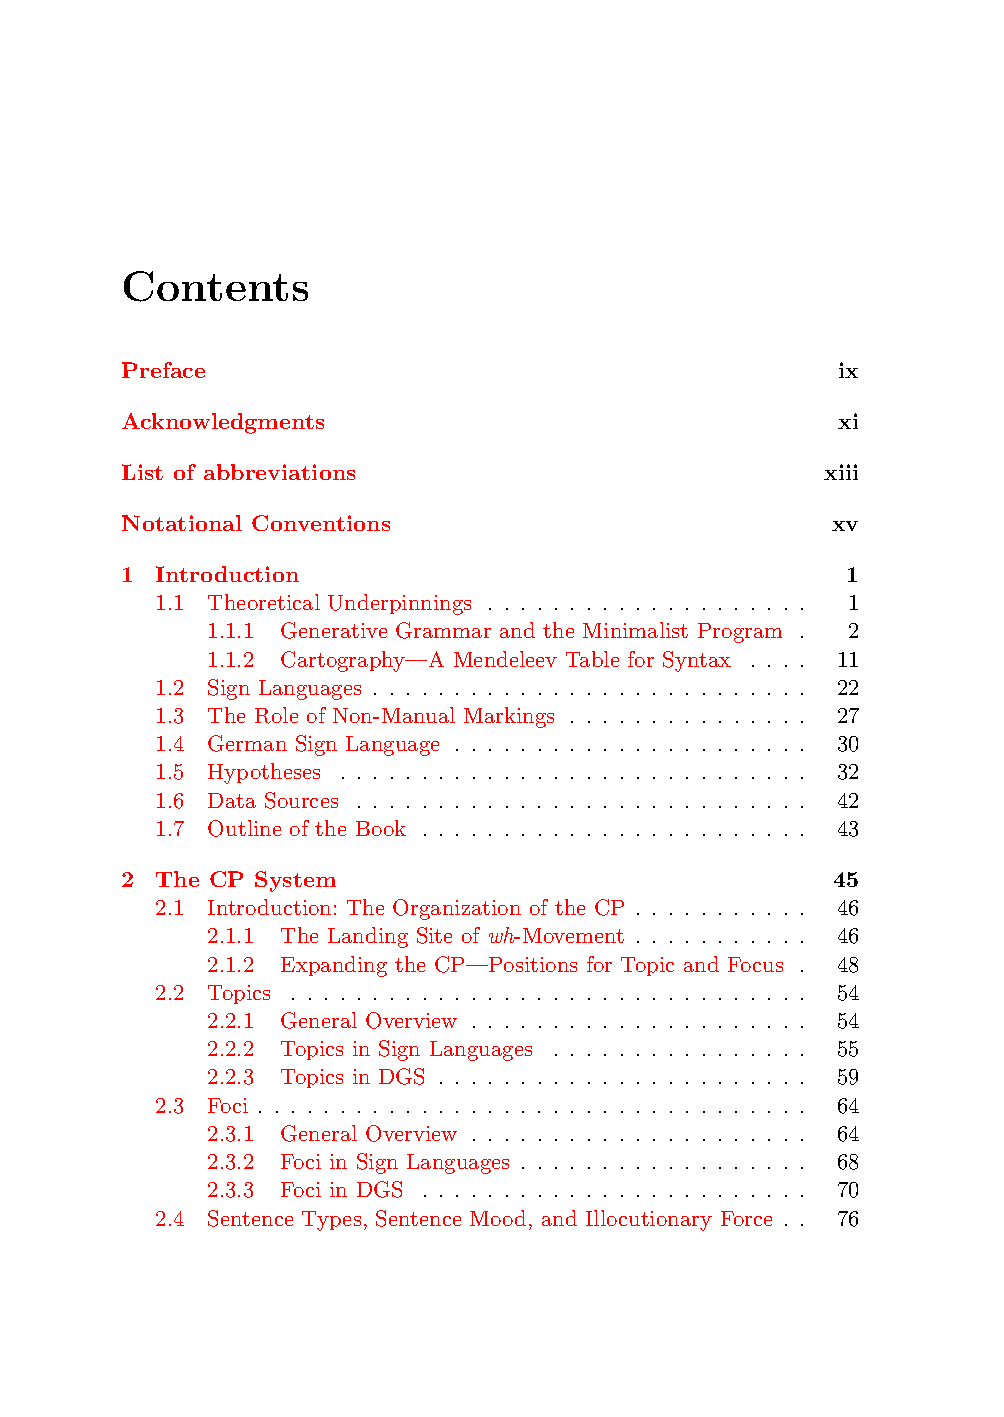
\includepdf[pages=1-6]{toc.pdf}

\section*{Content description}
\noindent The goal of the book is a hypothesis-based description of the clausal structure of German Sign Language (DGS). The structure of the book is based on the three clausal layers CP, IP/TP, and VoiceP. The main hypothesis is that scopal height is expressed iconically in sign languages: the higher the scope of an operator, the higher the articulator used for its expression (Bross \& Hole 2017). The book was written with two audiences in mind: On the one hand it addresses linguists interested in sign languages and on the other hand it addresses cartographers. As I do not assume that all sign language linguists have a background in Cartographic syntax and not all syntacticians to have a background in sign language linguistics, no background knowledge on either topic is required to read the book.

I will show that all high CP categories, i.\,e., the operators with highest scope, are expressed with the highest possible articulator, i.\,e., the eyebrows (or the eyes) in DGS. While the categories in the Rizzi hierarchy (e.\,g., sentence type encoding, topic, or focus) are exclusively expressed with the eyebrows, CP-categories in the Cinque hierarchy (e.\,g., epistemic modality) which still belong to the CP (as they are above T) are expressed either non-manually only or non-manually together with a manual adverb. The difference between the two possibilities is, as already hypothesized by Bross \& Hole (2017), a difference in meaning contribution: while non-manuals contribute not-at-issue meanings, manual signs express truth-functional content. Regarding the categories in the CP layer, the ones with highest scope are expressed with the eyebrows/eyes, while the lowest of these high categories (scalarity) is expressed with the cheeks---as expected by the main hypothesis. 

The categories inside the IP (below T), which consist of different modal flavors and the outer aspects, find manual expression. Manually marked adverbs generally concatenate from left to right---i.\,e., occur to the left of the VP. This strategy switches right before the VoiceP-internal categories as manner adverbs occur post-verbally. 

The categories inside the VoiceP, the inner aspects, also find manual expression, however, not through separate signs as with the outer aspects, but rather through manipulation of the movement path of the verb sign.\\


\noindent Bross, F. \& Hole, D. (2017a). Scope-taking strategies in German Sign Language. \textit{Glossa. A Journal of General Linguistics}, 2(1), 76.

\clearpage
\section*{Chapter abstracts}
\noindent \textbf{Chapter 1:} The first Chapter gives a brief overview of the theoretical frameworks for readers unfamiliar with Generative syntax and Cartography (as I assume that not all sign language linguists are familiar with that). Additionally, a short introduction into sign languages is presented (as I do not assume all interested readers are familiar with sign languages). Then, the basic structure of DGS is discussed followed by an outline of the book's hypotheses:

\begin{itemize}
	\item The Bodily Mapping Hypothesis (scopal relations are mapped onto the body):
	
	\begin{itemize}
		\item Categories above T are produced non-manually with the face by layering (first with the eyebrows then with the cheeks and the shoulders).
		\item Categories below T are produced manually by concatenation.
	\end{itemize}
	\item The at-issue/not-at-issue divide hypothesis: Categories above T contribute not-at-issue meaning, categories below T at-issue meaning. Thus, not-at-issue information is encoded non-manually while at-issue information is encoded manually.
	\item The Voice-P-internal modulation hypothesis: Categories inside the VoiceP (the inner aspects) are encoded by manipulation the movement path of the verb signs.
\end{itemize}

\noindent The last part of the chapter describes the data elicitation. The following three chapters are devoted to the higher CP layer (the `Rizzi domain'), the lower CP layer and the structure of the IP (the `Cinquean domain'), and the VoiceP.\\

\noindent \textbf{Chapter 2:} This chapter is devoted to the discussion of the expression of the higher CP categories. Here, I discuss topics and focus first. It is shown that two distinct types of topics exists in DGS, base-generated topics in a syntactically higher and moved topics in a syntactically lower position. Both topic types are marked non-manually with the upper face. Similarly, focus is marked non-manually with the upper face (although I show that focus marking is subject to dialectal variation). Then, I discuss the encoding of different sentence types in DGS (declaratives, polar interrogatives, constituent interrogatives, imperatives, and other sentence types).  It is shown that, similar to other sign languages, sentence types different from declaratives are marked non-manually with the upper face (only). The intensity peak of the non-manuals is always clause-final. Different modeling possibilities for the structures of the sentence types are also presented, e.\,g., to account for the clause-final intensity peak or the multitude of surface positions for \textit{wh}-signs.\\



\noindent \textbf{Chapter 3:} This chapter goes through the Cinquean categories. For the categories above tense it is shown that they are produced with upper-face non-manuals. However, different from the categories in Chapter 2, it is possible to additionally use a clause initial manual adverb (plus the non-manuals). Different from the Rizzi categories, the intensity peak of the non-manuals is clause-initial. Right above tense, the upper face stops to be the encoding device for the categories and the cheeks are used. While there is no grammaticalized tense in DGS, I show that the only known grammaticalized tense systems described for sign languages so far make use of the shoulders. Additionally, I present evidence that upper-face non-manuals only contribute not-at-issue meaning.

The categories below tense are all produces manually. The manual adverbs used in this domain all precede the VP. Adverb combinations are also discussed. In the case of modality, modal verbs show a great deal of flexibility in terms of positioning. However, data from combinations of different modal flavors shows that they are ordered in line with Cartographic principles. The only class of adverbs following the Vp are manner adverbs located right above the VoiceP. Thus, at this point, the (overt) scope-taking mechanisms switch in DGS. \\

\noindent \textbf{Chapter 4:} The goal of this (comparatively short) chapter is to show that the categories inside the VoiceP, the inner aspects, are not produced by facial non-manuals or by inserting manual signs, but by manipulating the movement path of the verb sign.\\

\noindent \textbf{Chapter 5:} In Chapter 5 I conclude the findings and briefly discuss the outcomes of each chapter and compare them to the hypotheses underlying the book.

\end{document}